\chapter{Oscilações Harmônicas: O Pêndulo Simples}
\label{chap:pendulo}

\section{Introdução}

Oscilações harmônicas aparecem em diversos sistemas físicos — desde massas em molas até circuitos elétricos oscilantes. O \textbf{pêndulo simples}, um sistema clássico da mecânica, é uma excelente porta de entrada para a modelagem de movimentos oscilatórios por meio de equações diferenciais lineares.

\section{Modelagem do Pêndulo Simples}

Considere uma massa $m$ presa a um fio ideal de comprimento $L$, oscilando sob a ação da gravidade.
A equação do movimento, obtida pela segunda lei de Newton projetada ao longo do arco, é:

\begin{equation}
    mL\od[2]{\theta}{t} + mg\sin\theta = 0
    \label{eq:pendulo-nao-linear}
\end{equation}

\section{Aproximação Harmônica}

Para pequenos ângulos ($\theta \ll 1$ rad), usamos a aproximação $\sin\theta \approx \theta$, e \eqref{eq:pendulo-nao-linear} se torna:

\begin{equation}
    \od[2]{\theta}{t} + \frac{g}{L}\theta = 0
    \label{eq:pendulo-linear}
\end{equation}

Essa é uma equação diferencial linear de 2ª ordem com solução geral:

\begin{equation}
    \theta(t) = \theta_0 \cos\left( \omega t + \varphi \right), \quad \text{com} \quad \omega = \sqrt{\frac{g}{L}}
\end{equation}

onde $\theta_0$ é a amplitude inicial e $\varphi$ a fase.

\section{Unidades e Exemplos Numéricos}

Assumindo $g = \qty{9.80665}{\meter\per\square\second}$ e um comprimento $L = \qty{1.00}{\meter}$, temos:

\[T = 2\pi \sqrt{\frac{\qty{1.00}{\meter}}{\qty{9.80665}{\meter\per\square\second}}} = \qty{2.006}{\second} \]

\section{Gráfico da Solução}

\begin{figure}[h]
    \centering
    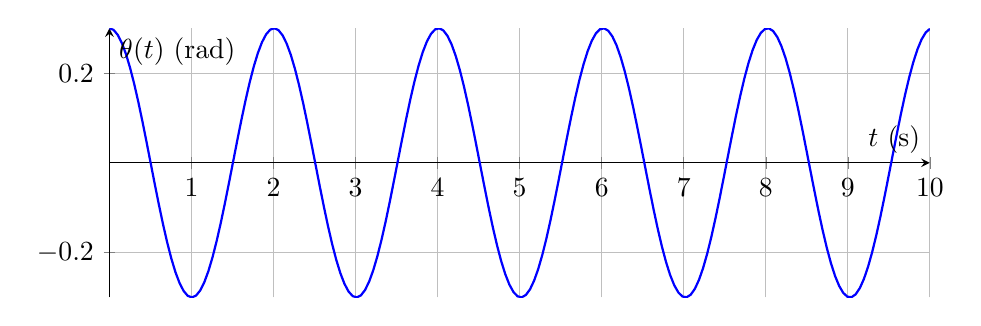
\begin{tikzpicture}
        \begin{axis}[
                width=12cm,
                height=5cm,
                xlabel={$t$ (s)},
                ylabel={$\theta(t)$ (rad)},
                grid=major,
                domain=0:10,
                samples=200,
                axis lines=middle
            ]
            \addplot[blue, thick] {0.3*cos(deg(2*pi*1/2.006*x))};
        \end{axis}
    \end{tikzpicture}
    \caption{Oscilação angular do pêndulo com $\theta_0 = 0{,}3$ rad.}
\end{figure}

\section{Discussão e Limitações}

A equação linearizada \eqref{eq:pendulo-linear} é válida apenas para pequenos ângulos. Para amplitudes maiores, a não linearidade introduz correções no período. Tais correções podem ser obtidas com expansões de série de Fourier ou integrais elípticas %\cite{Morin2008}.
